\subsection{Feldeffekt-Transistoren}

            \subsubsection{JFET Junction Field Effect Transistor}
            \begin{minipage}[T]{8cm}
                JFET als {\bf Konstantstromquelle}:\\
                benötigter Strom \fbox{$I_D = \frac{U_{GS}}{R_S}$}\\
                $U_{GS}$ entsprechend benötigem Strom aus Kennlinie lesen\\
                bei der Pinch-off-Grenze (Abschnürgrenze) sperrt der JFET
            \end{minipage}
            \begin{minipage}[T]{3.4cm}
                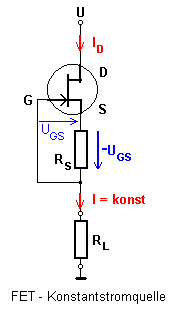
\includegraphics[height=4cm]{./images/JFETCCQuelle.png}
            \end{minipage}
            \begin{minipage}[T]{6cm}
                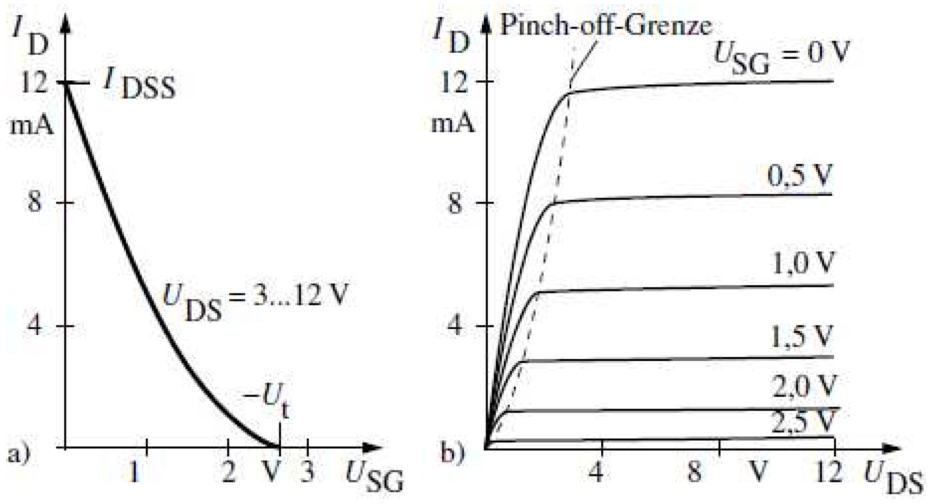
\includegraphics[height=4cm]{./images/JFETKennlinie.png}
            \end{minipage}
\hrule
            \subsubsection{MOSFET Metal Oxide Silicon Field Effect Transistor}
            \begin{minipage}[T]{6cm}
                \underline{Sperrbereich}\\\\
                $V_{GS} < V_{th} \to I_D = 0$\\
                typische $V_{th} = 0.5 \dots 1.5V$\\ 
                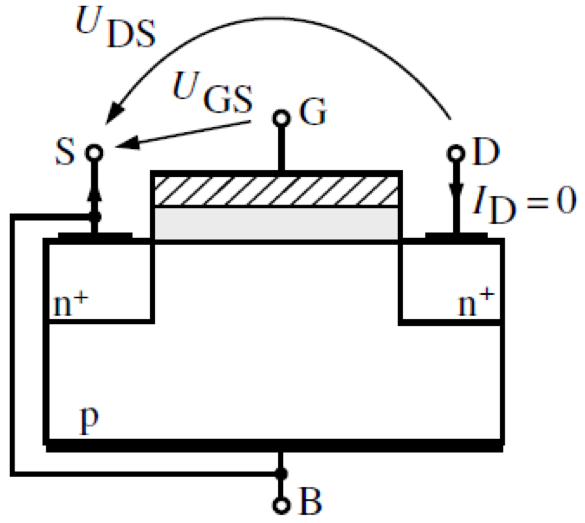
\includegraphics[height=4cm]{./images/MOSFETSperrbereich.png}
            \end{minipage}
            \begin{minipage}[T]{6cm}
                \underline{Widerstands-/Triodenbereich (linear)}\\\\
                $V_{GS} > V_{th} $ und $V_{DS}>0$\\
                $\to I_D$ fliesst\\
                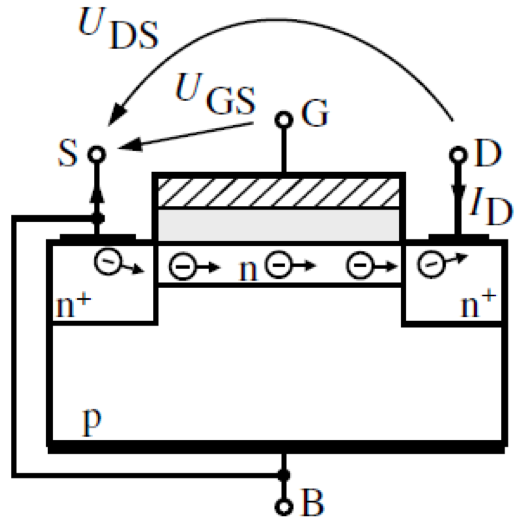
\includegraphics[height=4cm]{./images/MOSFETLinBereich.png}
            \end{minipage}
            \begin{minipage}[T]{6cm}
                \underline{S\"attigungs-/Pentodenbereich}\\\\
                $V_{DS} > V_{GS} - V_{th}$ Kanal wird abgeschnürt\\
                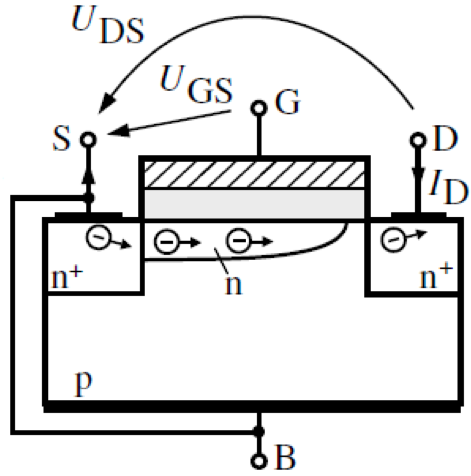
\includegraphics[height=4cm]{./images/MOSFETSaettBereich.png}
            \end{minipage}\\
            
            \subsubsection{Steuerkennlinien von verschiedenen MOSFETs}
            \begin{minipage}[T]{9cm}
                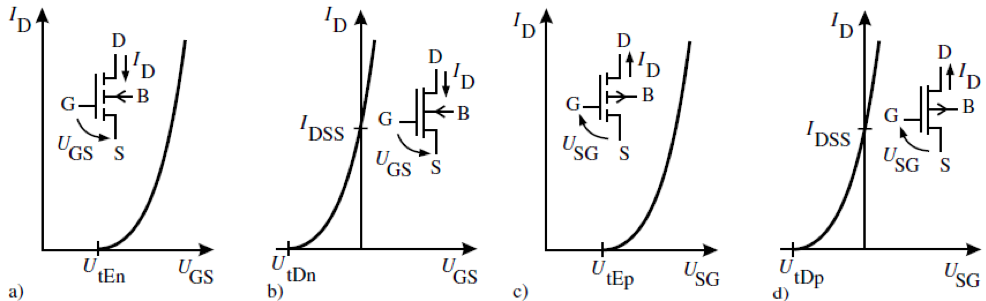
\includegraphics[height=2.4cm]{./images/MOSFETSteuerkennlinien.png}
            \end{minipage}
            \begin{minipage}[T]{9cm}
                a) n-Kanal Anreicherungs-Typ (selbstsperrend)\\
                b) n-Kanal Verarmungs-Typ (selbstleitend)\\
                c) p-Kanal Anreicherungs-Typ (selbstsperrend)\\
                d) p-Kanal Verarmungs-Typ (selbstleitend)\\
            \end{minipage}
                           
            \subsubsection{Berechnung des Drainstromes $I_D$}
            \begin{minipage}{13cm}
                $I_D = \begin{cases}
                0                       & $für $ V_{GS} \leqq V_{th}\\
                {\bf Sperrbereich}\\\\
                
                \beta\cdot(V_{GS} - V_{th})^2\cdot(1 + \lambda\cdot V_{DS})    &  $
                für $ 0\leqq V_{GS} - V_{th} \leqq V_{DS}\\
                {\bf Pentodenbereich} $ PB Sättigungsbereich $\\\\
                
                \beta\cdot(2(V_{GS}-V_{th})V_{DS} - V_{DS}^2)\cdot(1 + \lambda\cdot V_{DS}) &  $
                für $ 0\leqq V_{GS} - V_{th} \geqq V_{DS}\\
                {\bf Triodenbereich} $ TB linearer Bereich$
                
                \end{cases}$\\
                
                \begin{tabular}[t]{l l l}
                    $b$: Kanalbreite & $L$: Kanallänge & $\mu_n$: Leitfähigkeit Kanal\\
                    $\epsilon_{ox}$: Dielektrizität Oxidschicht & $\lambda$: Pinch-off-Konstante & $d_{ox}$: Oxiddicke\\
                    $V_{th}$: Threshold-Spannung & $\beta$: Steilheitsparameter & $K$: Steilheitskoeffizient
                \end{tabular}
            \end{minipage}
            \vrule \hspace{0.1cm}
            \begin{minipage}[T]{6cm}
                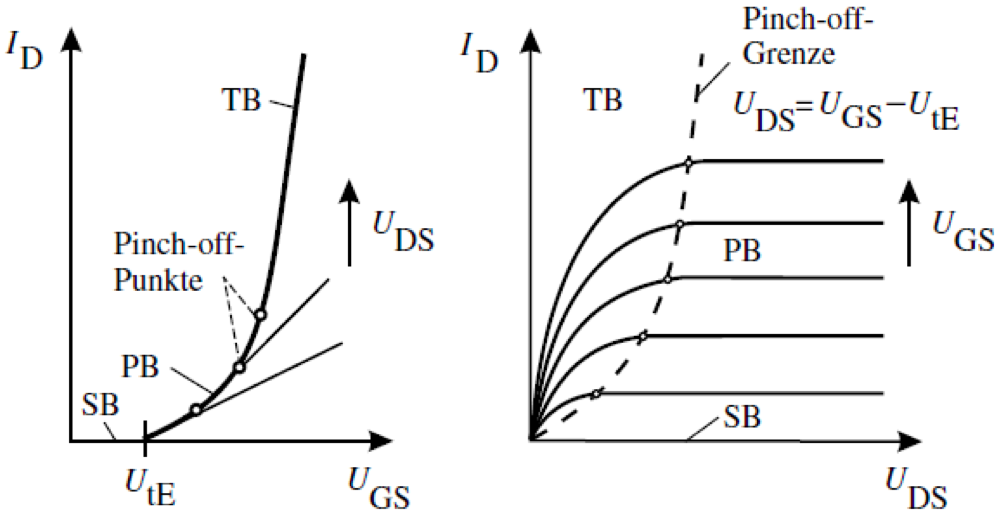
\includegraphics[width=6cm]{./images/MOSFET_IU_Kennlinie.png}\\
                \vspace{0.8cm}\\
                Steilheitsparameter \hspace{1mm}\fbox{$\beta = \frac{K}{2} = \frac{\mu_n \epsilon_{ox}}{2d_{ox}}\frac{b}{L}$}
            \end{minipage}\\
            
            \subsubsection{Kleinsignalmodell des MOSFET}
            \begin{minipage}[T]{10.5cm}
                Steilheit
                \hspace{29.3mm}\fbox{$S = g_m = 2\beta(V_{GS}-V_{th}) = \sqrt{4\beta\cdot I_D}$}\\
                Ausgangsleitwert
                \hspace{15.9mm}\fbox{$g_d = \beta\lambda(V_{GS}-V_{th})^2$}\\
                Drain-Source-Widerstand
                \hspace{3mm}\fbox{$r_{DS} = \frac{1}{\lambda\cdot I_{D0}}$}\\
                Gate-Source-Spannung
                \hspace{7mm}\fbox{$V_{GS} \cong \sqrt{\frac{I_D}{\beta}} + V_{th}$}
            \end{minipage}
            \begin{minipage}[T]{3.5cm}
                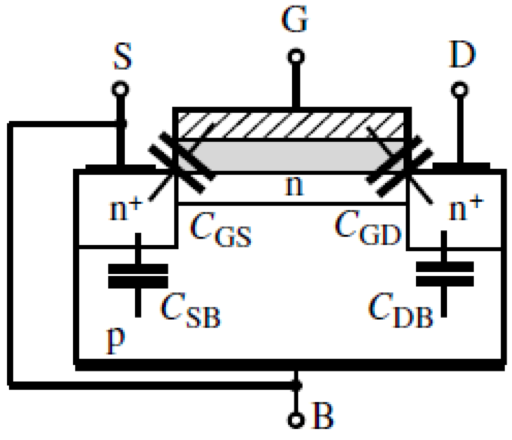
\includegraphics[width=3cm]{./images/MOSFET_Aufbau.png}
            \end{minipage}
            \begin{minipage}[T]{5cm}
                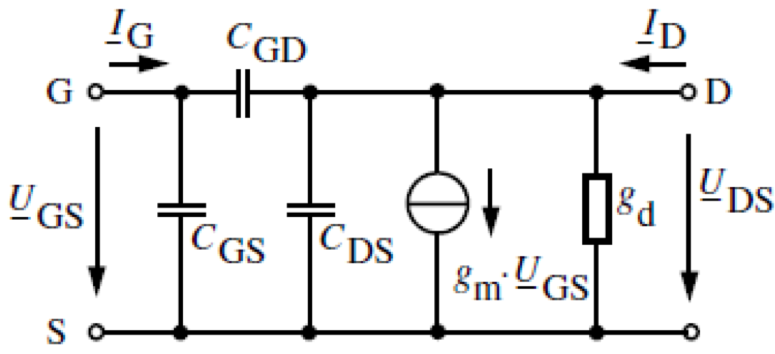
\includegraphics[width=5cm]{./images/MOSFET_Ersatzsch.png}
            \end{minipage}
\vspace{1mm}\hrule
            \subsubsection{Differenzverstärker}
            \begin{minipage}[T]{14cm}
                Ausgangswiderstand
                \hspace{10.6mm}\fbox{$r_{out} = R//r_{DS}$}\\
                Verstärkung
                \hspace{23.3mm}\fbox{$A_D = -\frac{S}{2} \cdot R$}\\
                Ausgansdifferenzspannung
                \hspace{1.7mm}\fbox{$V_{out_{diff}} = A \cdot V_{in_{diff}}$}
                
            \end{minipage}
            \begin{minipage}[T]{5cm}
                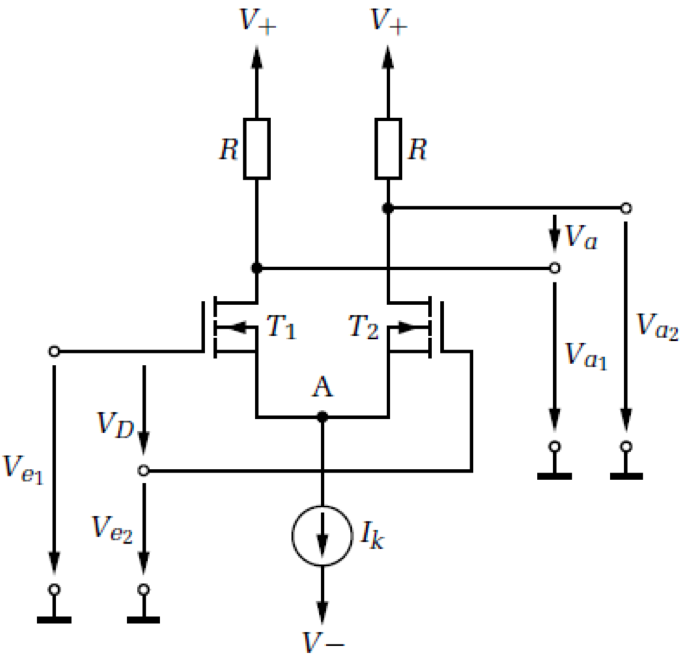
\includegraphics[height=4cm]{./images/MOSFET_Diffamp.png}
            \end{minipage}